\section{Proof-of-Concept Implementation}
\label{sec:evaluation}

\subsection{Illustrative \crossflow Implementation}
\begin{figure}[t]
  \centering
  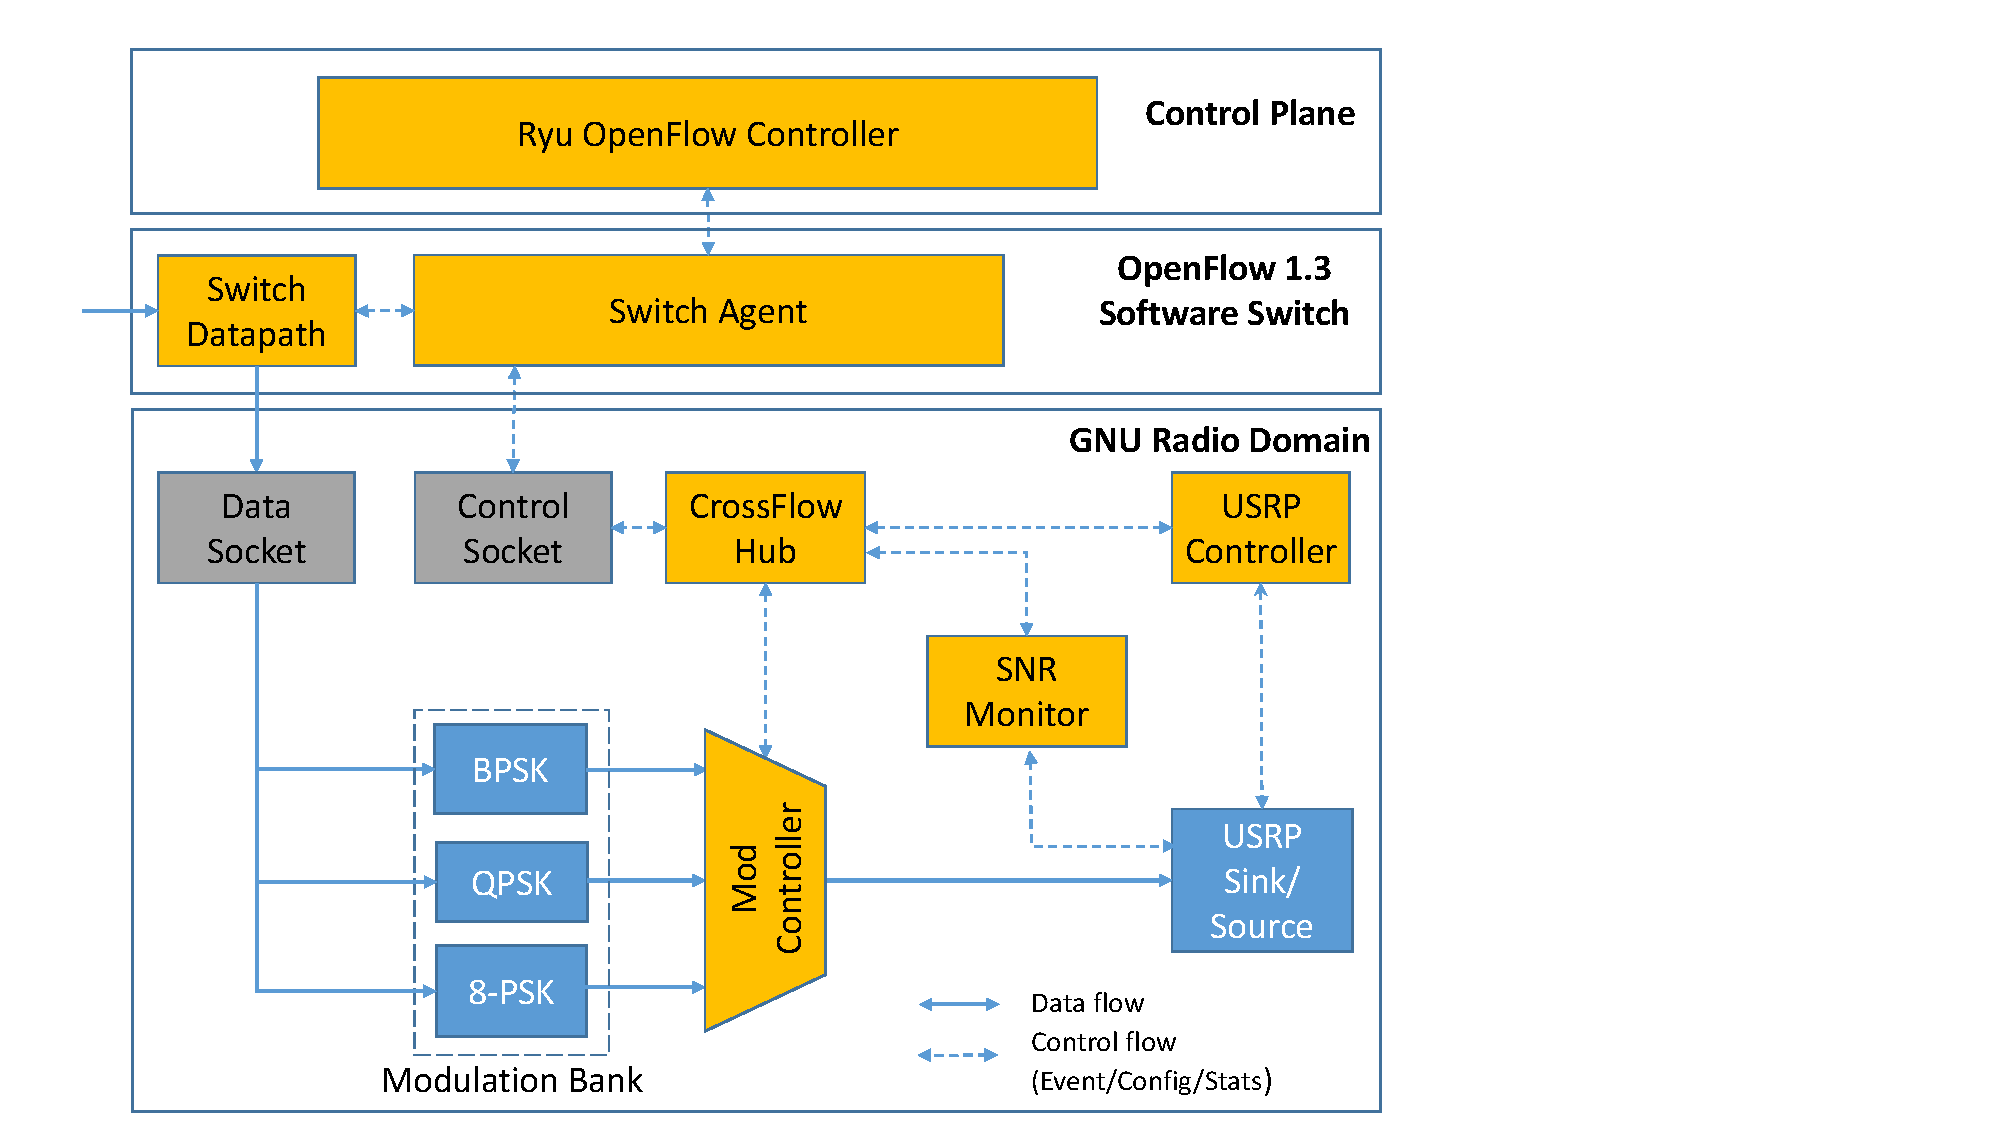
\includegraphics[width=0.6\textwidth]{figures/Flowgraph.pdf}
  \caption{Transmitter implementation diagram of \crossflow with two processing blocks: Sink and Modulators}
  \label{fig:flowgraph}
\end{figure}

In this section, we describe our implementation of \emph{adaptive modulation}, \emph{frequency hopping} and \emph{cognitive radio} applications using the \crossflow framework. For illustration, we implement our model on a USRP N210 SDR from Ettus Research. We use the CPqD Softswitch~\cite{ofsoftswitch13} (\texttt{ofsoftswitch}) software as the switch agent in the SDN model. Its main functionality is to enable communication between GNU Radio and the python based Ryu SDN controller. As described in previous sections, the applications will send messages to the processing blocks, e.g., to configure them. The \texttt{ofsoftswitch} then forwards this request to a centralized \texttt{\crossflow Hub} inside the GNU Radio domain. 

There are four main components (blocks) in the illustrative \crossflow module, as given in Figure~\ref{fig:flowgraph},that we implement in GNU Radio, namely, the \texttt{\crossflow Hub}, the Modulation Controller (Mod Controller for brevity), the SNR Monitor and the USRP Controller.
\begin{itemize}
\item The \texttt{\crossflow Hub} is the interface between the Mod and USRP controllers in GNU Radio and the Ryu SDN controller. The \texttt{\crossflow Hub} and the Ryu SDN controller communicate via Socket PDU. The \texttt{\crossflow Hub} is responsible for receiving commands from \texttt{ofsoftswitch} (or any other compliant interface), interpreting the commands, and forwarding the commands to the appropriate controller block (i.e., either the USRP controller or Mod controller in our implementation). It is also responsible for receiving information from different controller blocks and sending information to the Ryu SDN controller. The \texttt{\crossflow Hub} has in/out ports to send commands and receive information to/from the GNU radio controller blocks. It also has in/out PDU ports for interfacing with Socket PDU.
\item The \texttt{Mod Controller} is one of the main controllers in the design. It is responsible for receiving commands from the \texttt{\crossflow Hub}, and selecting the appropriate modulation scheme from the modulation bank. For illustration, we include three modulation schemes in our modulation bank (BPSK, QPSK, and 8PSK); however, thanks to the modular design, we can easily add more schemes. The Mod Controller can also feedback information to the Ryu SDN controller about the modulation scheme that is currently in use and the number of modulation schemes available in the modulation bank.
\item The \texttt{SNR Monitor} is responsible for monitoring the SNR level and generating an event in case the SNR level falls below a certain threshold, which can be configured by the application. Currently the framework uses the existing SNR probe of GNU Radio, which supports four $M$-PSK SNR estimators. This monitoring block is also responsible for relaying the SNR statistics back to \texttt{\crossflow Hub} in response to a SNR statistics query generated by the application.
\item The \texttt{USRP Controller} is responsible for controlling different RF parameters of the USRP Transmitter/Receiver based on commands from the \texttt{\crossflow Hub}. In our proof-of-concept implementation, we control the carrier frequency and the power of the signal. It can also feedback information to the \texttt{\crossflow Hub} about the current RSSI, temperature, SNR, carrier frequency, power, etc.
\end{itemize}
Although our illustrative implementation only has three controllers (one facilitating abstraction of the USRP Sink/RF implementation, the other facilitating abstraction of SNR estimation and another one facilitating abstraction of the adaptive modulation implementation), additional controllers can be easily added to support new applications, functionalities, and abstractions.

\subsection{Example Applications}
%\begin{figure*}
%\centering
%  \begin{subfigure}[b]{\textwidth}
%  	\centering
%      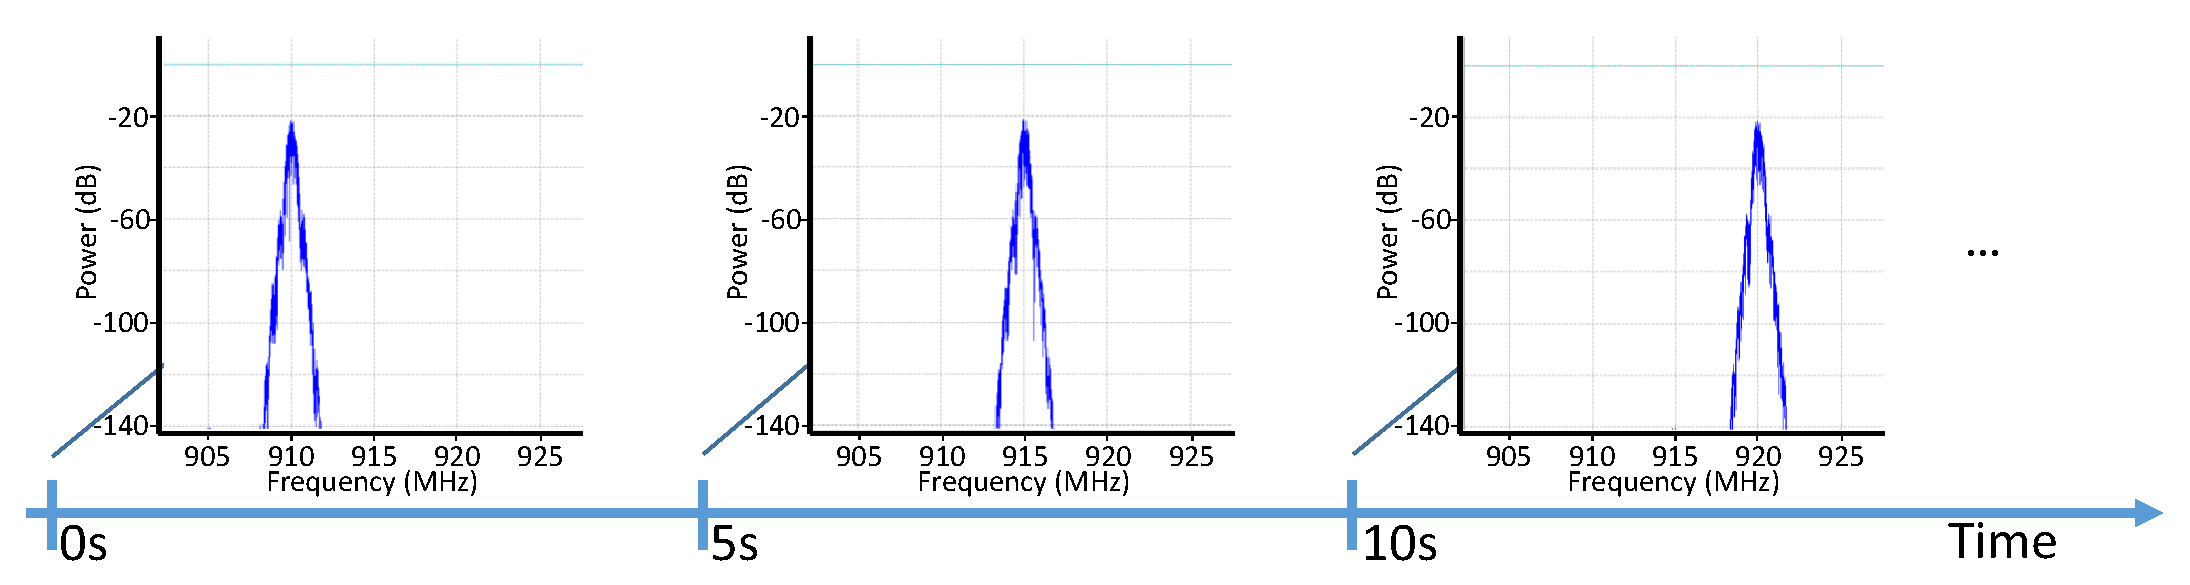
\includegraphics[width=0.9\textwidth]{figures/Freq.pdf}
%      \caption{Spectral output for \emph{frequency hopping} application. The frequency changes every 5 seconds keeping BPSK as a fixed modulation scheme.}
%      \label{fig:freq}
%  \end{subfigure}
  
%  \begin{subfigure}[a]{\textwidth}
%  \centering
%      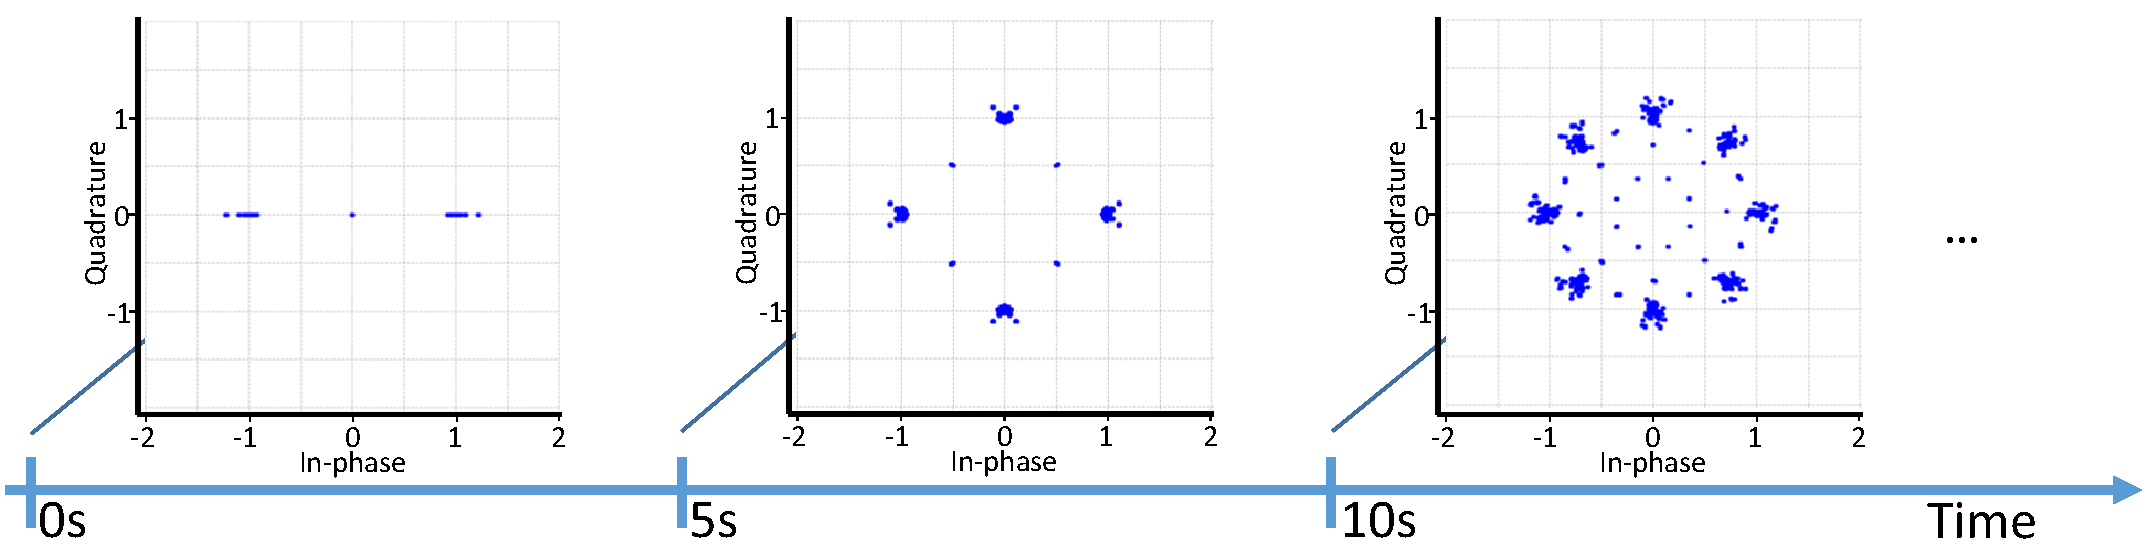
\includegraphics[width=0.9\textwidth]{figures/Mod.pdf}
%      \caption{Constellation output for \emph{adaptive modulation} application. The modulation scheme changes every 5 seconds keeping a fixed frequency of 910 MHz.}
%      \label{fig:mod}
%  \end{subfigure}%
%  \caption{Experimentation results  \emph{frequency hopping} and \emph{adaptive modulation}}
%\end{figure*}

\begin{figure}[t]
  \centering
  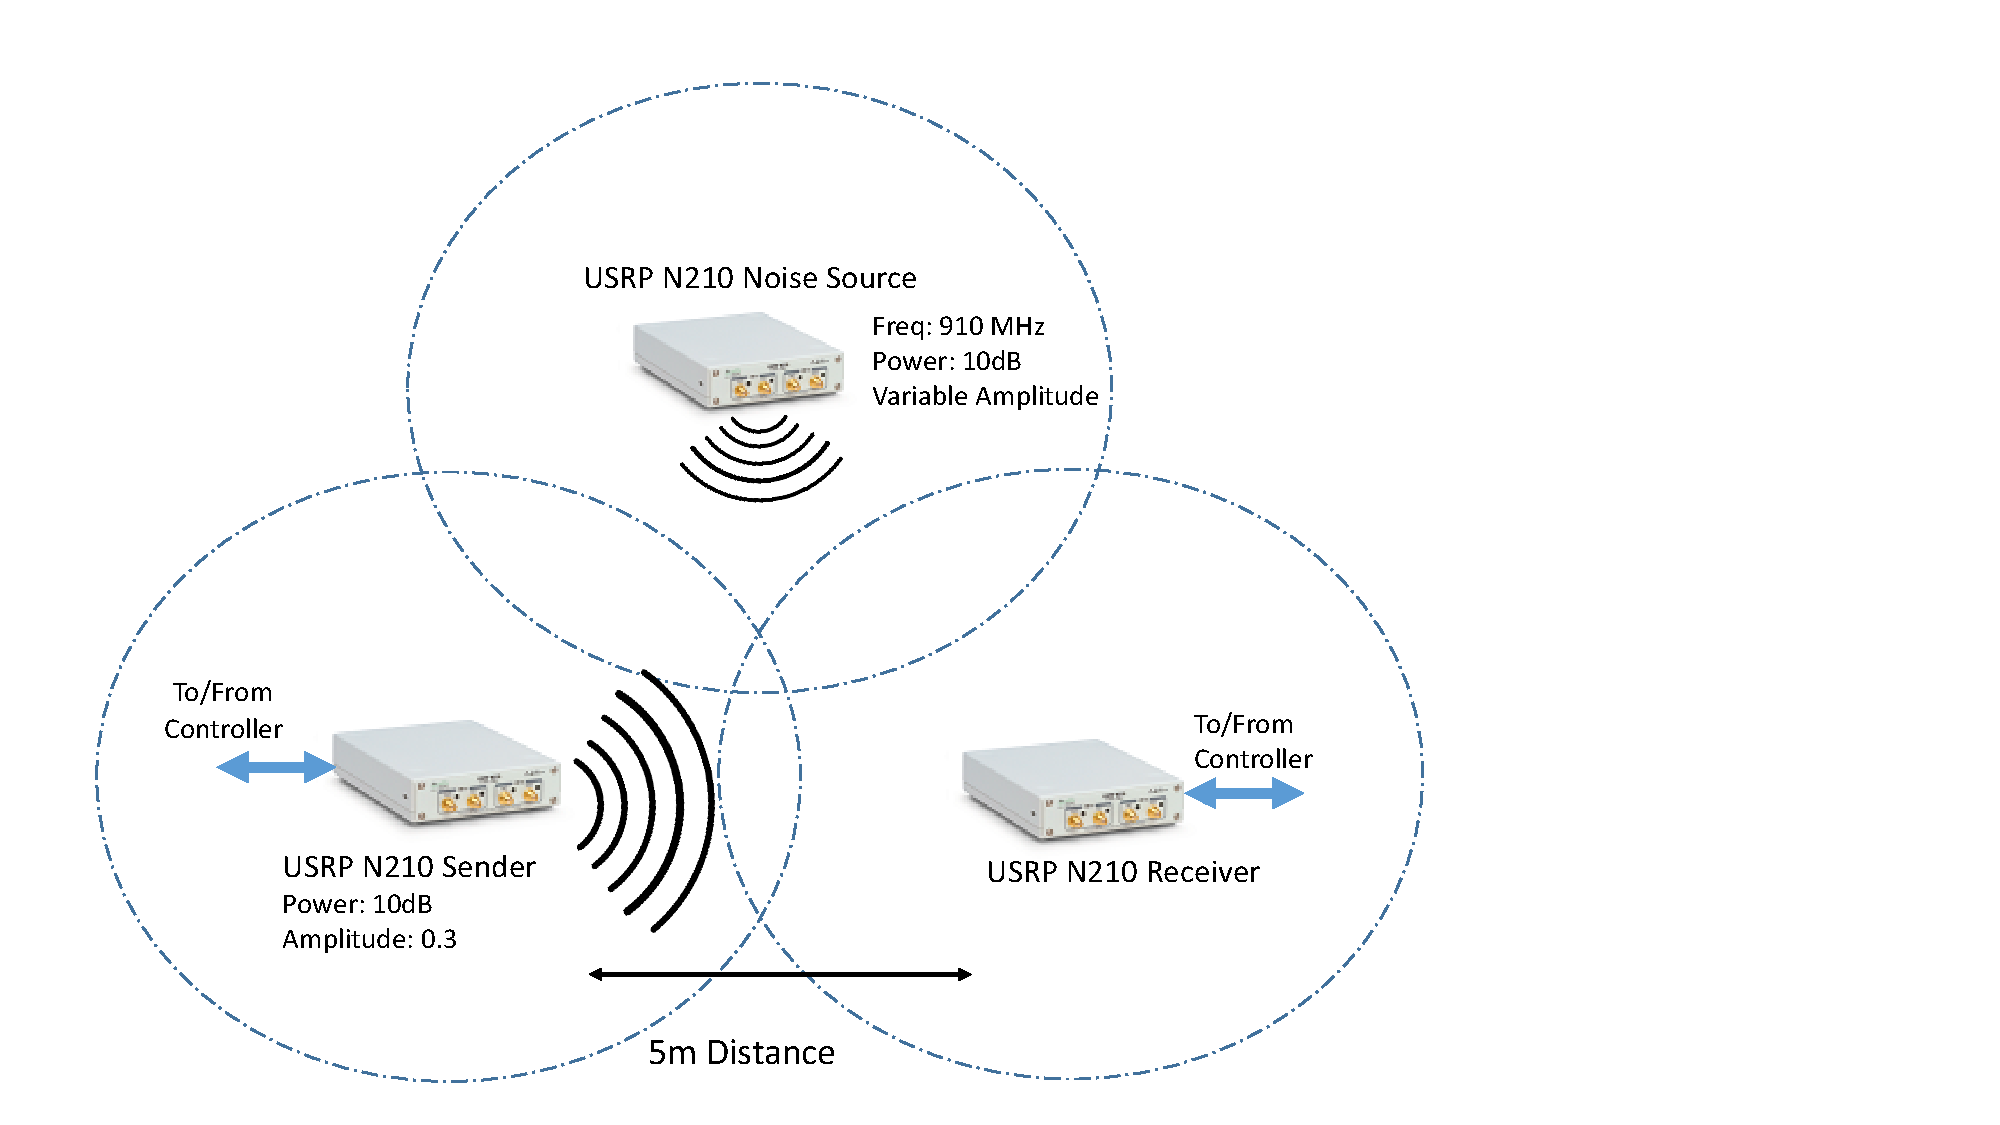
\includegraphics[width=0.6\textwidth]{figures/Setup.pdf}
  \caption{Setup for cognitive radio application in \crossflow}
  \label{fig:setup}
\end{figure}

\begin{figure}[t]
  \centering
  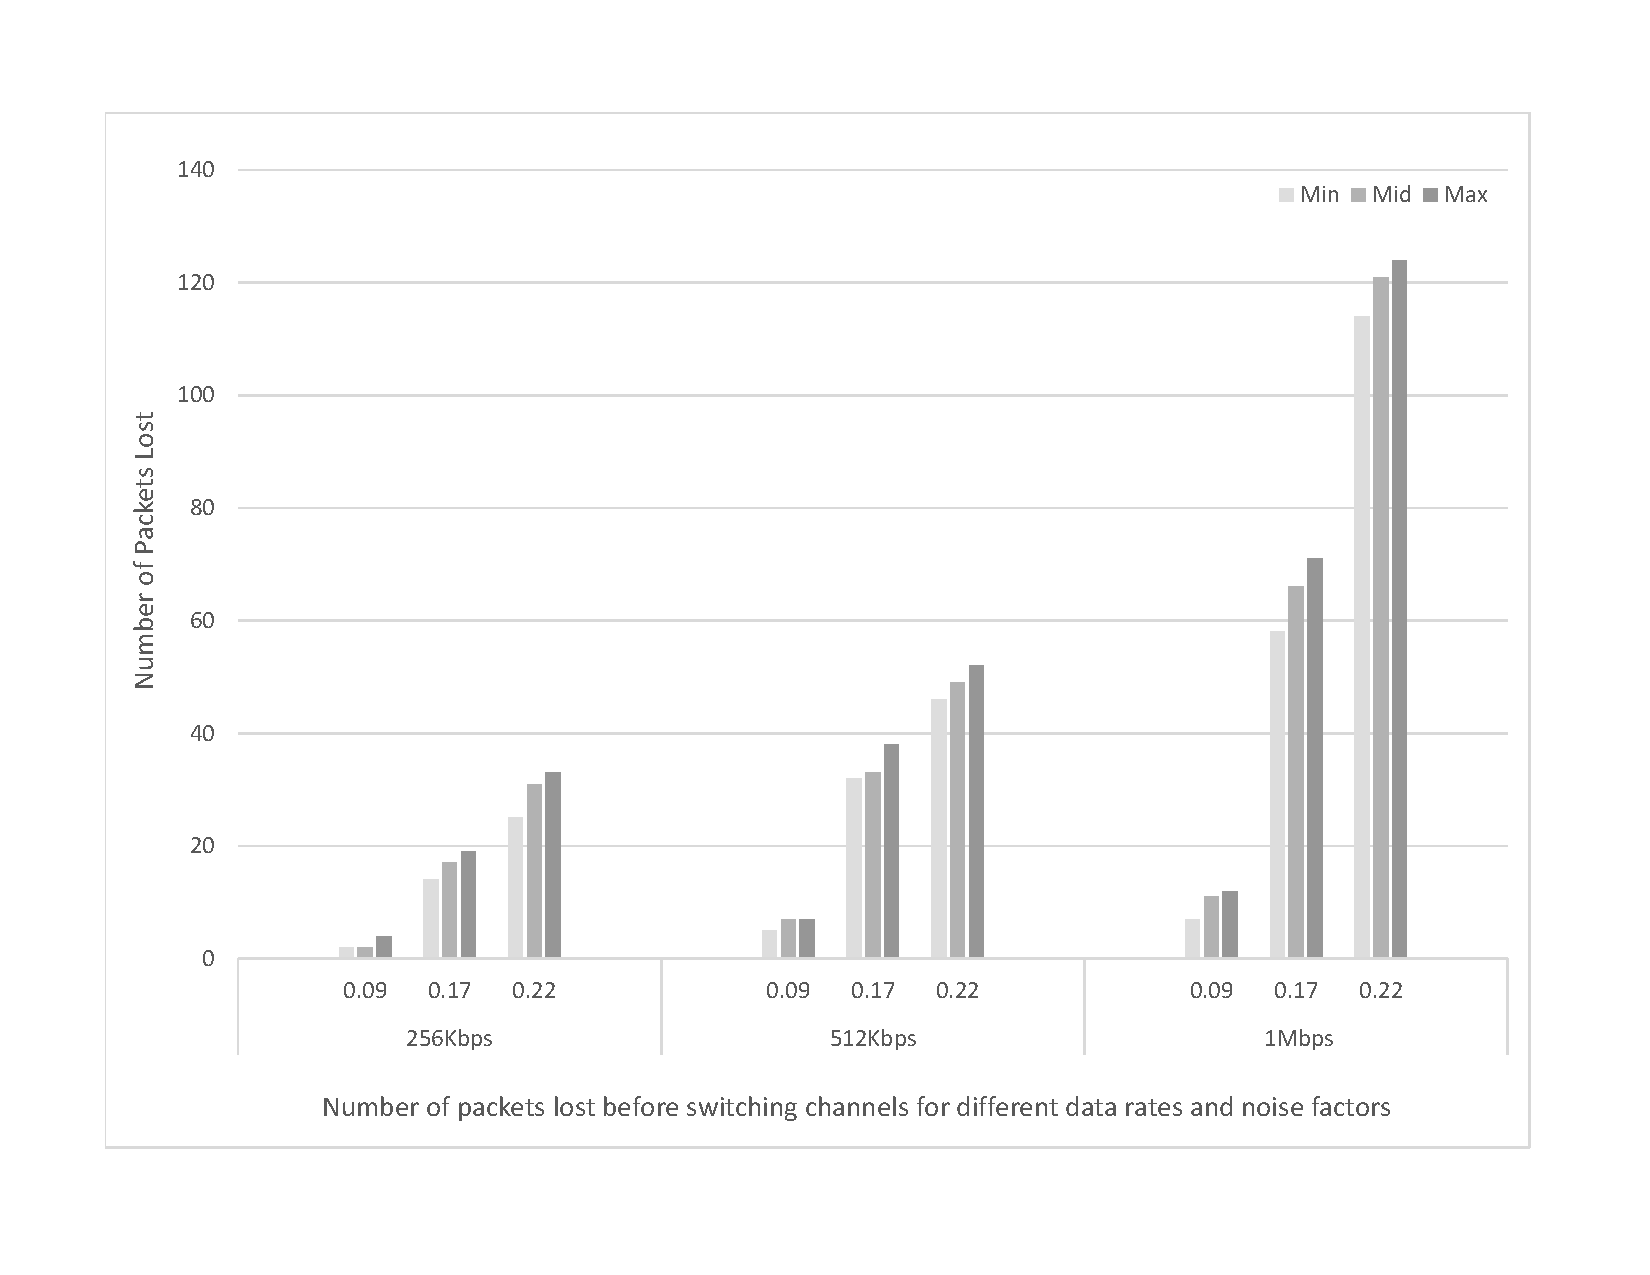
\includegraphics[width=0.5\textwidth]{figures/Overhead.pdf}
  \caption{Range of packets loss while changing channels by keeping a fixed data rate and a varying noise factor across each experiment}
  \label{fig:overhead}
\end{figure}

% \begin{figure}[t]
%   \centering
%   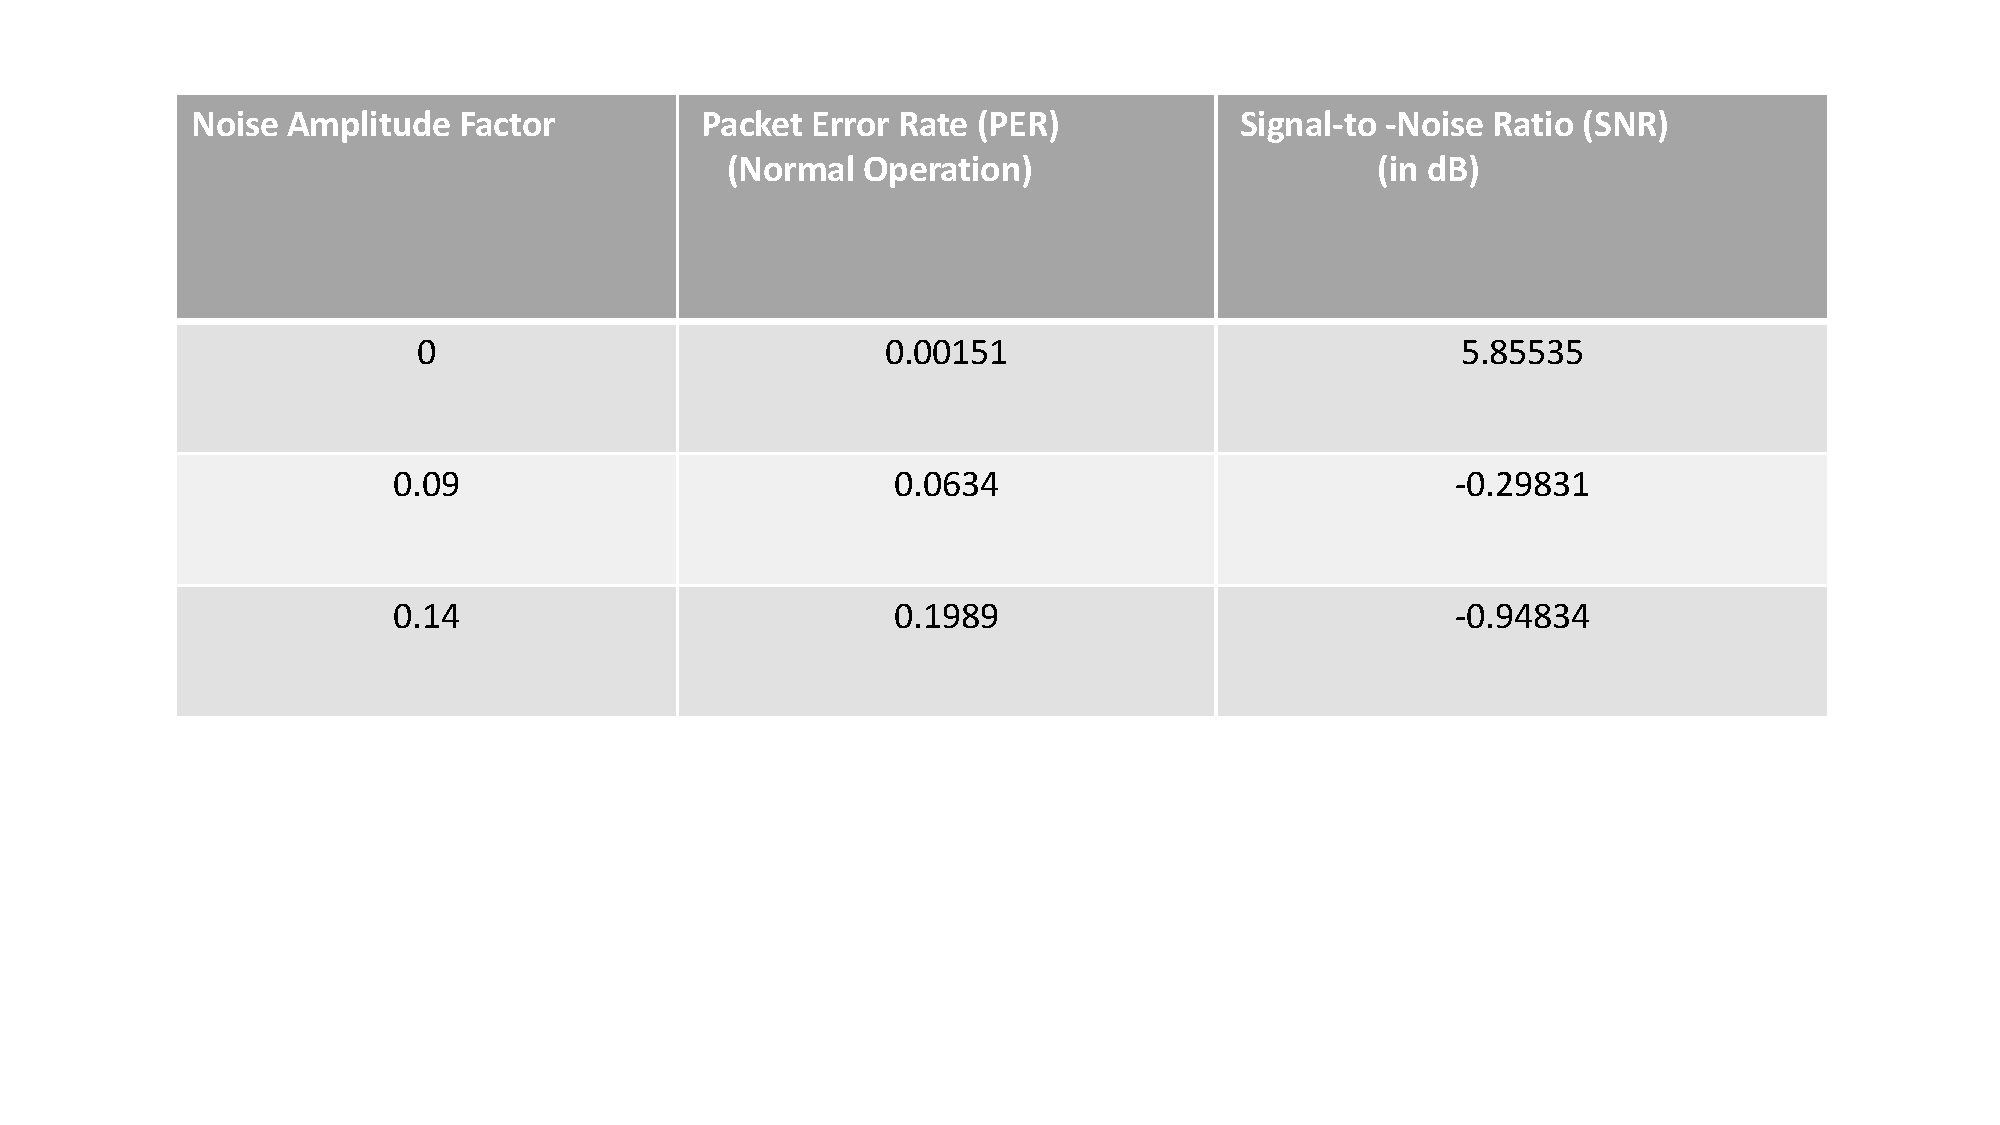
\includegraphics[width=0.5\textwidth]{figures/Table.pdf}
%   \caption{Variation of SNR and PER with increasing Noise Amplitude Factor keeping a fixed data rate of 1Mbps. }
%   \label{fig:table}
% \end{figure}

% Please add the following required packages to your document preamble:
% \usepackage{booktabs}
\begin{table}[]
\centering
\caption{Variation of SNR and PER with increasing Noise Amplitude Factor keeping a fixed data rate of 1Mbps.}
\label{my-label}
\begin{tabular}{@{}|c|c|c|@{}}
\toprule
Noise Amplitude Factor & Packet Error Rate & SNR (in dB) \\ \midrule
0                      & 0.15\%            & 5.8553                     \\ \midrule
0.09                   & 6.34\%            & -0.2983                    \\ \midrule
0.14                   & 19.89\%           & -0.9483                    \\ \bottomrule
\end{tabular}
 \label{fig:table}
\end{table}



\subsubsection{Frequency Hopping Application}
Frequency hopping is a technique of transmitting radio signals by spreading the signal over a sequence of changing frequencies. It can be used against jamming and for protecting against unauthorized eavesdropping. 
%For implementation, the receiver of the signal must be aware of the sequence of frequencies so that it can tune into the appropriate channel. This requires synchronization between the transmitter and the receiver. In \crossflow, we implement this application easily as only the controller needs to be aware about the predetermined sequence. This sequence can even be dynamic according to the channel conditions and policies. 
In our implementation, the Ryu SDN controller simply issues a \emph{GNU-CONFIG-FREQ} command with the desired frequency and pushes this configuration to the device. 
As shown in Figure~\ref{fig:flowgraph}, the \texttt{ofsoftswitch} receives this command and forwards it to the GNU Radio domain. The centralized \texttt{\crossflow Hub} inside the GNU Radio domain processes this request and issues appropriate commands to the  USRP Controller, which ultimately signals the USRP block to tune into the requested frequency. 
%For this experiment, the application toggles among a pre-determined sequence of 910, 915 and 920MHz frequencies every 5 seconds along with a fixed BPSK modulation scheme.

\subsubsection{Adaptive Modulation Application}
Adaptive Modulation is a technique where the modulation is changed according to the conditions of the channel. There are various estimators which are used for obtaining channel quality. These can be Signal-to-noise ratio (SNR), Bit error rate (BER) and other environment specific estimators. 
%For illustration, we assume a fixed sequence for changing the modulation schemes every 5 seconds.
Similar to the \emph{frequency hopping} application, the Ryu SDN controller issues the \emph{GNU-CONFIG-MOD} command with the appropriate modulation scheme (BPSK, QPSK, or 8PSK) and forwards the request to the device. The request ultimately reaches the Mod Controller, which is a multiplexer block as shown in Figure~\ref{fig:flowgraph}, that selects the requested modulation scheme. 
%In this experiment, the application changes the modulation scheme between BPSK, QPSK and 8PSK every 5 seconds, keeping a fixed carrier frequency of 910 MHz.

\subsection{Cognitive Radio Application}
We build upon the frequency hopping application mentioned above to construct a cognitive radio application. Cognitive radio is a type of radio in which the device is aware of its environment and can dynamically change its operating parameters like transmission power, frequency, gain etc in response to changing environmental conditions. In \crossflow, we implement an application that can configure a radio device to switch channels based upon a low SNR event measured by the device. The experimental setup is shown in Figure~\ref{fig:setup}, where we have three USRP N210 devices that act as sender, receiver and noise source. The sender is set at a 10 dB power level and 0.3 transmission amplitude factor, while the noise source is set at 10 dB power with a variable amplitude factor. Note that the amplitude factor is simply a constant that is multiplied to the transmitted signal to adapt the effective transmission power. The sender and receiver are at a distance of 5 meters apart and the sender begins transmission at 910 MHz carrier frequency with 1 Mbps data rate and packet length of 50 Bytes. The noise source on the other hand, sends high frequency pulses with varying amplitude factors at 910 MHz frequency. We refer to the noise source's transmission amplitude factor as the noise amplitude factor (NF). When SNR falls below a specified threshold, a low SNR event is triggered by the \texttt{SNR Monitor} block and the event summary is sent to \texttt{ofsoftswitch} through \texttt{\crossflow Hub}. This request is then forwarded to the Ryu SDN controller using the event response message. The application, upon receiving this message, sends a {GNU-CONFIG-FREQ} command so that the device changes the channel to the requested frequency. The sequence of actions involved in changing the channel is similar to the one mentioned in the previous section for \emph{frequency hopping}.

Using this setup, we conduct two tests: one to measure the effect of the NF on the receiver's packet error rate (PER) and SNR at the 910 MHz carrier frequency (both measured over 1,000,000 packets transmitted at 1 Mbps with NFs of 0.0, 0.09, 0.14), and another to measure how quickly the cognitive radio can trigger and respond to a low SNR event (with NFs 0.09, 0.17 and 0.22, and data rates 256 Kbps, 512 Kbps and 1 Mbps).
Table~\ref{fig:table} shows the PER and SNR values obtained in the first experiment. As expected, the PER increases and SNR decreases with increasing NFs. 
In the second experiment, which demonstrates a simple cognitive radio application, the transmitter and receiver pair switch to a new carrier frequency (915 MHz) when the instantaneous received SNR falls below the pre-defined 6 dB threshold. In Figure~\ref{fig:overhead}, we show the number of packets that are lost over the course of time required for the SNR to be sensed below the 6 dB threshold, for the receiver to generate the low SNR event, and for the Ryu SDN controller to respond by issuing the {GNU-CONFIG-FREQ} command, and finally for the transmitter to switch frequencies. We repeat this experiment three times for each combination of data rate and noise factor, and plot each measurement in Figure~\ref{fig:overhead} as a separate bar. %These to send In order to determine the overhead for signaling and switching channels, we ran the experiment again with varying Noise Amplitude Factor of 0.09, 0.17 and 0.22 for each fixed data rates of 256 Kbps, 512 Kbps and 1 Mbps. The result of this experiment is shown in Figure~\ref{fig:overhead} which indicates that packet loss for changing channels increases with increasing data rates, but it in mainly in the order of a hundred packets per million packets. This shows that our design for such a programmatic radio using centralized co-ordination is viable and it serves as a base for the development of sophisticated applications.
